%%%%%%%%%%%%%%%%%%%%%%%%%%%%%%%%%%%%%%%%%
% Medium Length Graduate Curriculum Vitae
% LaTeX Template
% Version 1.1 (9/12/12)
%
% This template has been downloaded from:
% http://www.LaTeXTemplates.com
%
% Original author:
% Rensselaer Polytechnic Institute (http://www.rpi.edu/dept/arc/training/latex/resumes/)
%
% Important note:
% This template requires the res.cls file to be in the same directory as the
% .tex file. The res.cls file provides the resume style used for structuring the
% document.
%
%%%%%%%%%%%%%%%%%%%%%%%%%%%%%%%%%%%%%%%%%

%----------------------------------------------------------------------------------------
%	PACKAGES AND OTHER DOCUMENT CONFIGURATIONS
%----------------------------------------------------------------------------------------

\documentclass[margin, 10pt]{res-short} % Use the res.cls style, the font size can be changed to 11pt or 12pt here

\usepackage{helvet} % Default font is the helvetica postscript font
%\usepackage{newcent} % To change the default font to the new century schoolbook postscript font uncomment this line and comment the one above
\usepackage[UTF8]{ctex}


\usepackage{hyperref}
\hypersetup{
    colorlinks=true,
    linkcolor=blue,
    filecolor=magenta,      
    urlcolor=cyan,
}
\urlstyle{same}

\usepackage{etaremune,amsmath,amssymb,graphicx,wrapfig}

\setlength{\textwidth}{5.1in} % Text width of the document
\setlength{\sectionskip}{.1in}

\newsectionwidth{0.8in}
\hoffset 0.4in

\begin{document}

%----------------------------------------------------------------------------------------
%	NAME AND ADDRESS SECTION
%----------------------------------------------------------------------------------------

%\moveleft.5\hoffset\centerline{\huge\bf 宋 茂源 \;\textbar\; Maoyuan `Raymond' Song} % Your name at the top
 
%\moveleft\hoffset\vbox{\hrule width 6.5in height 1pt}\smallskip % Horizontal line after name; adjust line thickness by changing the '1pt'
 
%\moveleft.5\hoffset\centerline{普渡大学 计算机科学系} % Your address
%\moveleft.5\hoffset\centerline{305 N. University St, West Lafayette, IN 47907}
%\begin{wrapfigure}{R}{0.25\textwidth} %this figure will be at the right
%    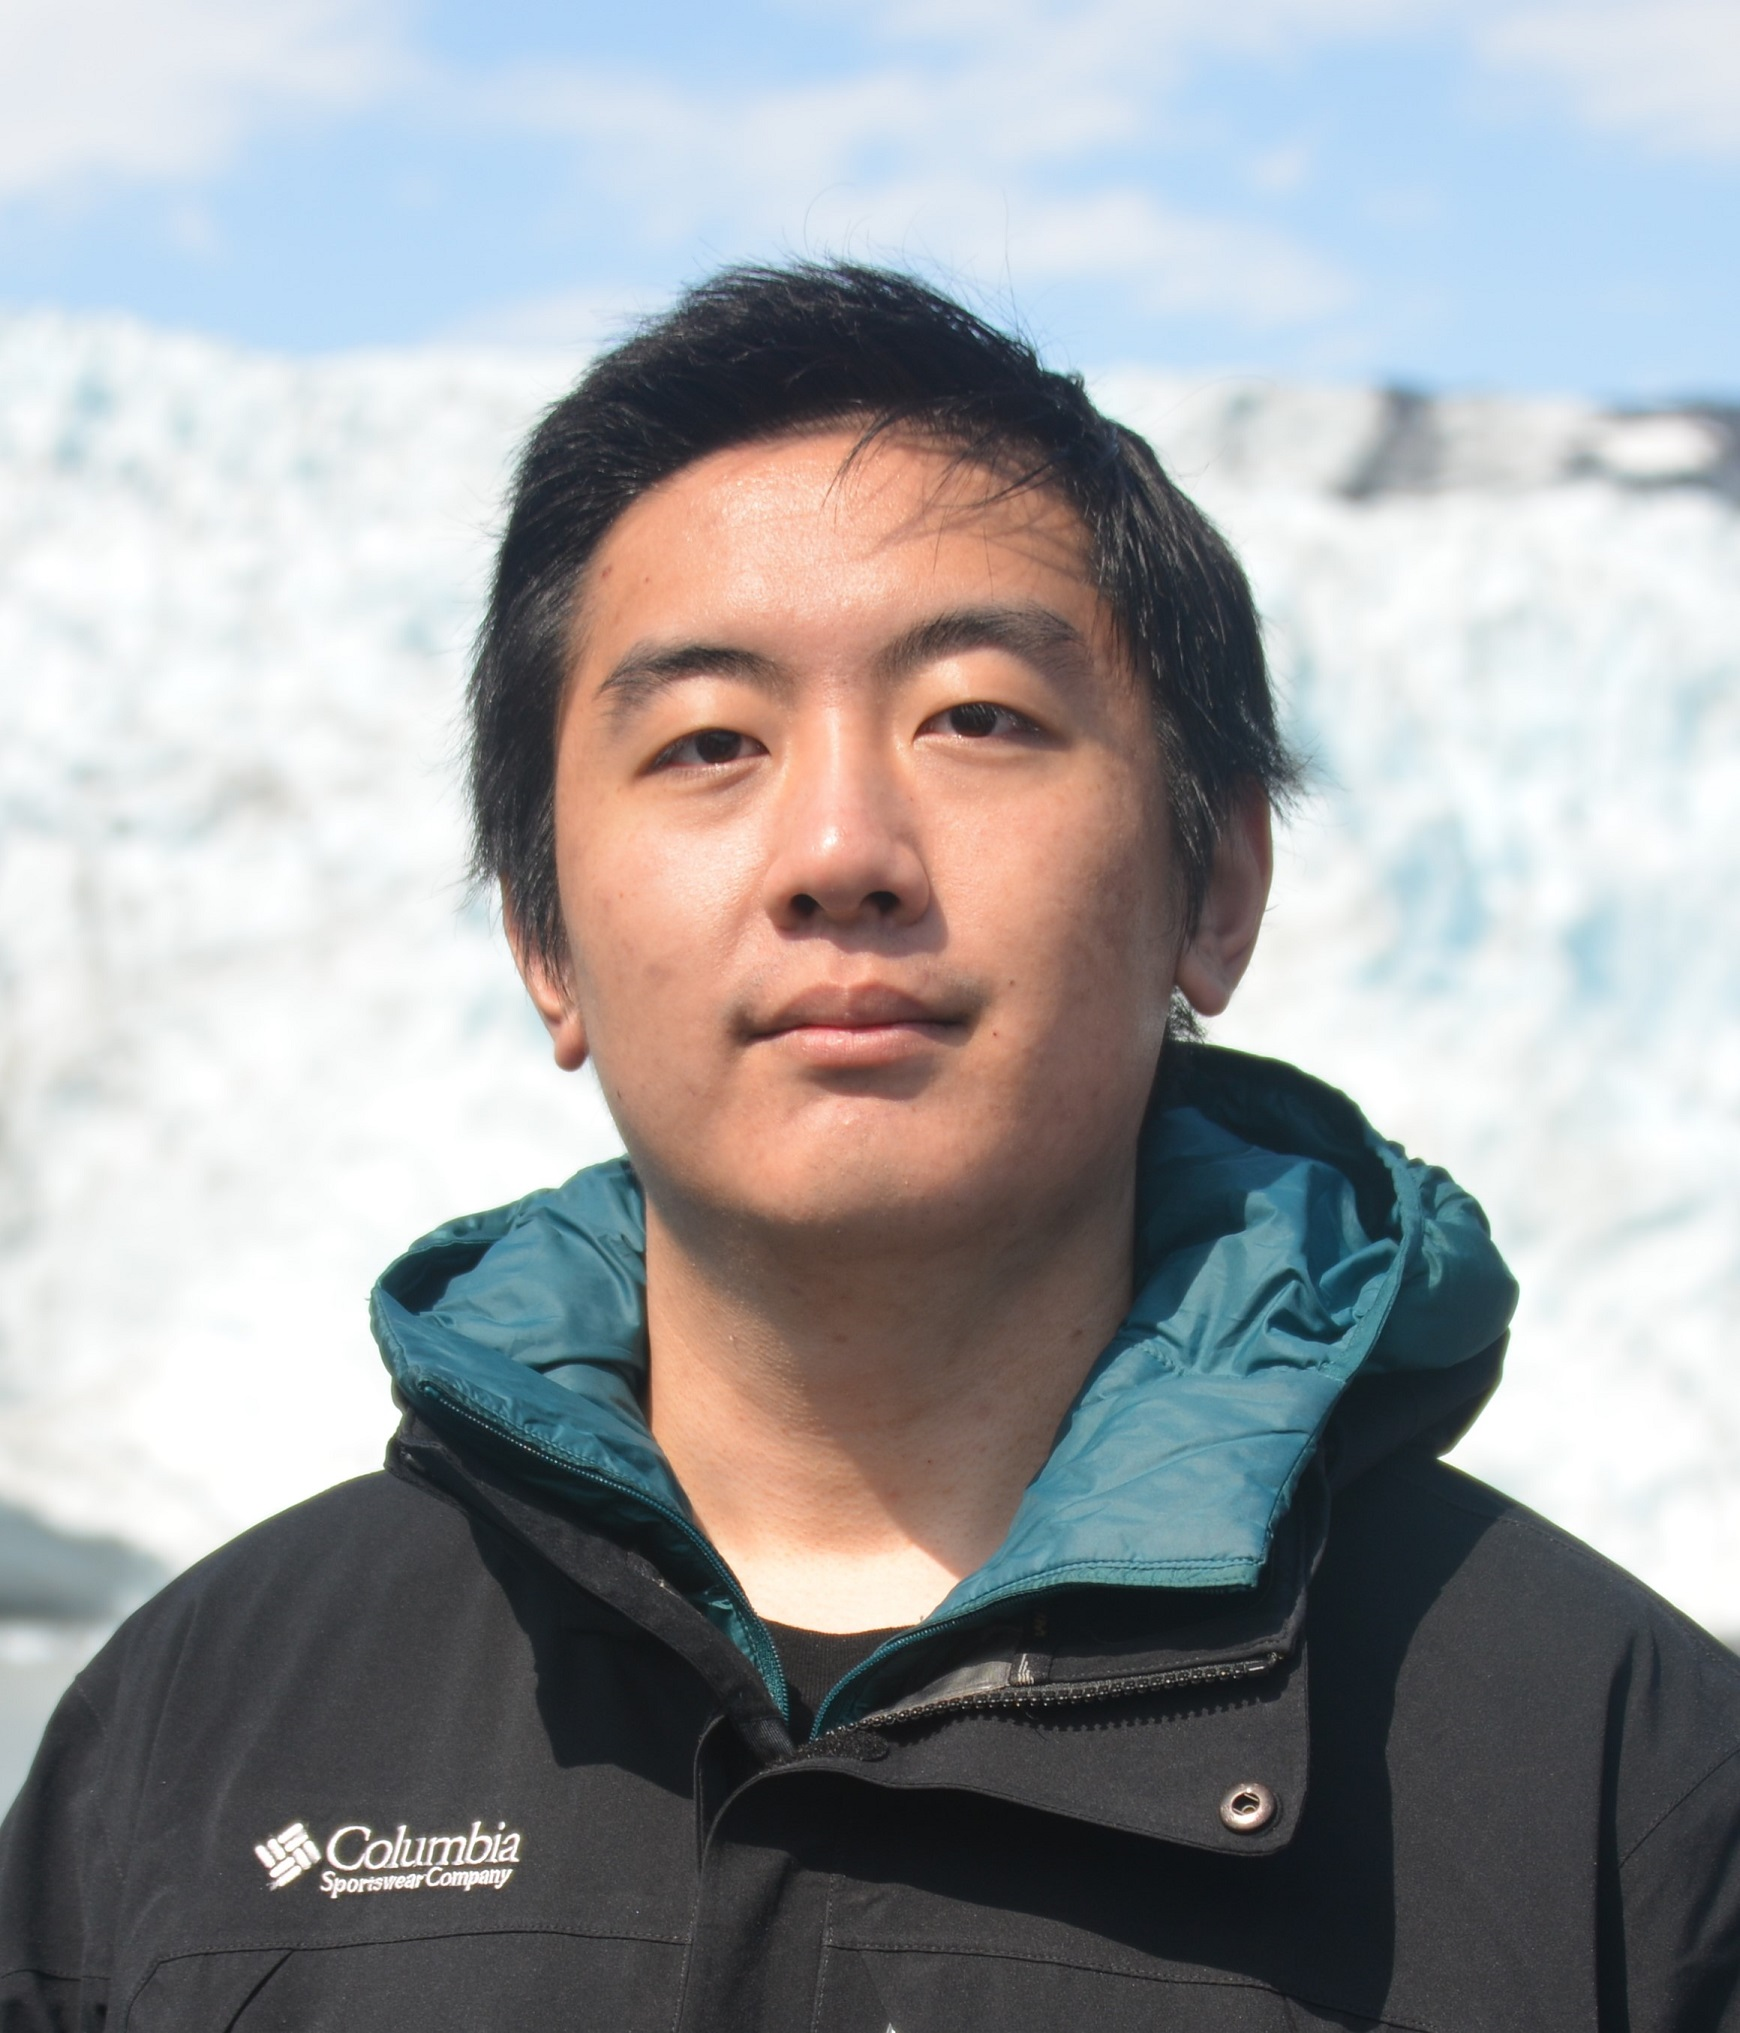
\includegraphics[width=0.25\textwidth]{pic.jpg}
%\end{wrapfigure}

\moveleft2\hoffset\leftline{{\huge\bf 宋 茂源 \;\textbar\;} {\large Maoyuan `Raymond' Song}} % Your name at the top
 
\moveleft2\hoffset\vbox{\hrule width 5in height 1pt}\smallskip % Horizontal line after name; adjust line thickness by changing the '1pt'
\moveleft2\hoffset\leftline{出生年月: 2000年1月 \;\qquad\; 性别: 男}
\moveleft2\hoffset\leftline{普渡大学\;科学院\;计算机科学系\;博士在读}


%----------------------------------------------------------------------------------------

\begin{resume}

\section{联系方式}
\emph{微信}: maoyuans\\
\emph{电子邮箱}: MaoyuanRS@gmail.com\\
\emph{个人主页}: \href{https://maoyuans.github.io}{maoyuans.github.io}

 
\section{研究方向}  

在线算法 (Online algorithm): 在线线性规划, 在线覆盖与装箱规划, 求解器; \\
学习理论 (Learning theory): 在线学习, 列表学习;\\
次线性算法 (Sublinear algorithms): 数据流算法;\\
学习增强算法 (Learning-augmented algorithm); 统计估计 (Statistical estimation); 计算复杂性理论 (Computational complexity); 超越最坏情况分析 (Beyond worst-case analysis).

热爱并擅长机器学习, 人工智能, 与传统算法的交叉领域内的研究课题: 如何用传统算法辅助机器学习与人工智能, 及如何用机器学习方法辅助传统算法, 以解决理论及应用问题. 熟练掌握Python, C, C++, LaTeX, Java, Git等编程语言. 

\section{教育经历}

{\bf 普渡大学}\; 科学院\; 计算机科学\; 博士在读 \hfill 2020年8月 -- \hphantom{202008000}
\begin{itemize}
\item 导师: Elena Grigorescu 和 Paul Valiant. 已通过博士资格开题考试. 预计2025年5月毕业.
\item 主要课程: 机器学习理论 (Machine Learning Theory), 密码学 (Cryptography), 次线性算法 (Sublinear Algorithms), 随机算法 (Randomized Algorithm), 计算复杂度理论 (Theory of Computation).
\end{itemize} 

{\bf 卡耐基梅隆大学}\; 计算机科学院\; 计算机科学\; 硕士学位 \hfill 2019年5月 -- 2020年5月
\begin{itemize}
\item 导师: Carleton Kingsford. \hspace{-2em}
\item 论文题目: Linear Time Addition of Fibonacci Encodings.\\
研究如何用线性时间在不解码的情况下将斐波那契编码求和。
\end{itemize} 

{\bf 卡耐基梅隆大学}\; 计算机科学院\; 计算机科学\; 学士学位 \hfill 2015年8月 -- 2019年5月
\begin{itemize}
\item 辅修专业: 离散数学与逻辑.
%\item 校级优秀毕业生 (University Honors).
\item 主要课程: 算法设计与分析 (Algorithm Design \& Analysis), 机器学习 (Machine Learning), 谱图论 (Spectral Graph Theory), 集合论 (Set Theory), 极值组合学 (Extremal Combinatorics).
\end{itemize} 

{\bf 北京市第八中学超常儿童教育实验班} (北京八中少儿班) 17班 \hfill 2010年9月 -- 2014年6月 

%\section{实习经历}

%{\bf 资深成员,项目内容负责人} \hfill 2018年1月 - 2020年5月 \\
%Carnegie Mellon University Computer Science Academy \hfill 美国宾夕法尼亚州匹兹堡

%\begin{itemize}
%\item 作为资深项目成员参与卡内基梅隆大学计算机学院的CMU Computer Science Academy项目。Computer Science Academy是一个由计算机学院官方资助的非盈利性组织,致力于为美国高中的学生与教师提供高效且便捷的计算机科学教育资源。
%\item 设计并管理项目内容,包括但不限于课程练习,质量保证,和教育工作者支持资源。
%\end{itemize} 


\section{已发表论文}
{\it 遵循理论计算机科学领域惯例, 文章作者按照姓氏首字母排序.}
\begin{enumerate}
\item 一个应用于优化目标为凹函数的在线装箱规划的简洁学习增强算法.\\
A Simple Learning-Augmented Algorithm for Online Packing with Concave Objectives.\\
Elena Grigorescu, Young-San Lin, {\bf Maoyuan Song}.\\
\emph{收录于arXiv预印文库 2406.03754, 2024.}
\item 均值估算的最优性: 超越最坏情况分析, 超越次高斯表现, 超越$1 + \alpha$阶动差.\\
Optimality in Mean Estimation: Beyond Worst-Case, Beyond Sub-Gaussian, Beyond $1 + \alpha$ Moments.\\
Trung Dang, Jasper C.H. Lee, {\bf Maoyuan Song}, Paul Valiant.\\
\emph{发表于 Conference on Neural Information Processing Systems (NeurIPS) 2023}.
\item 应用于在线线性与半正定规划的学习增强算法.\\
Learning-Augmented Algorithms for Online Linear and Semidefinite Programming.\\
Elena Grigorescu, Young-San Lin, Sandeep Silwal, {\bf Maoyuan Song}, Samson Zhou.\\
\emph{发表于 Conference on Neural Information Processing Systems (NeurIPS) 2022},\\
\emph{被选为重点展示 (Spotlight presentation)}.
\item 斐波那契编码的线性时间求和.\\
Linear Time Addition of Fibonacci Encodings.\\
{\bf Maoyuan (Raymond) Song}.\\
\emph{硕士论文, 2020}.
%\item Application of Convolutional Neural Networks in Accent Identification.\\
%Kevin Chionh, {\bf Maoyuan Song}, Yue Yin.\\
%\emph{Project Report} (2018).
\end{enumerate}

\section{待发表论文}
\begin{enumerate}
\item 应用于优化目标为凸函数的在线覆盖规划的学习增强算法.\\
Learning-Augmented Algorithms for Online Covering Programs with Convex Objectives.\\
Elena Grigorescu, Young-San Lin, {\bf Maoyuan Song}. %\\
\emph{2024.}
\item 一维实数轴上的通用均值估算: 最优次高斯表现, 耐错性, 与重尾分布表现.\\
All-Purpose Mean Estimation over $\mathbb{R}$: Optimal Sub-Gaussianity with Outlier Robustness and Low Moments Performance.\\
Jasper C.H. Lee, Walter McKelvie, {\bf Maoyuan Song}, Paul Valiant. %\\
\emph{2024.}
\end{enumerate}

%\section{实习经历}

\section{受邀参与的\\访问项目}
%{\it 受邀参与的访问项目}\\
{\bf 加州大学伯克利分校 Simons计算理论学院} \hfill 2024年1月 -- 2024年3月
\begin{itemize}
\item 受邀作为访问学者参与了``纠错编码: 理论与实践'' (Error-Correcting Codes: Theory and Practice) 的项目研究.
\end{itemize}

\section{受邀开设的\\专题讲座}
%{\it 受邀开设的专题讲座}
应用于学习增强算法的简单调换策略.\\
(Simple Switching Strategies for Learning-Augmented Algorithms.)
\begin{itemize}
\item 芝加哥大学/丰田工业大学芝加哥分校\;学习增强算法\;专题座谈会, 2024年8月.
\end{itemize}

均值预测下的超越最坏情况分析.\\
(Beyond Worst-Case Optimality in Mean Estimation.)
\begin{itemize}
\item Conference on Neural Information Processing Systems (NeurIPS), 2023年12月.
\item 卡耐基梅隆大学\;理论计算机午餐讲座, 2023年9月.
\item 罗格斯大学/DIMACS\;计算理论讲座, 2023年9月.
\item 西北大学\;理论计算机讲座, 2023年7月.
\end{itemize}

应用于在线线性与半正定规划的学习增强算法.\\
(Learning-Augmented Algorithms for Online Linear and Semidefinite Programming.)
\begin{itemize}
\item Conference on Neural Information Processing Systems (NeurIPS), 2022年12月.
\end{itemize}
%\item Learning-Augmented Algorithms for Online General Covering LPs.\\
%Theory Reading Group at Purdue, 2022年11月.
%\item On `The Primal-Dual Method for Learning Augmented Algorithms'.\\
%Theory Reading Group at Purdue, February 2022.
%\item On `PROPm Allocations of Indivisible Goods to Multiple Agents'.\\
%Theory Reading Group at Purdue, November 2021.
%\item Online Facility Location Problem with Recourse.\\
%Theory Reading Group at Purdue, 2021年3月.
%\item Fields and Polynomials, based on 15-751 TCS Toolkit.\\
%Advanced Algorithm Reading Group at Purdue, October 2020.
%\item Fast Multiplication using Discrete Fourier Transform, based on 15-751 TCS Toolkit.\\
%Advanced Algorithm Reading Group at Purdue, September 2020.
%\item Linear Time Addition of Fibonacci Encodings.\\
%硕士论文答辩, 2020年4月.

\section{其他\\实习经历}
%{\it 其他实习经历}\\
{\bf 卡耐基梅隆大学 Kingsford实验室} \hfill 2018年5月 -- 2018年8月
\begin{itemize}
\item 参与开发和优化{\it Salmon}软件, 该软件旨在使用机器学习进行快速基因分析排序. 使用NVIDIA的并行计算库CUDA简化并加速不同基因序列之间的配对算法. 
\end{itemize}

{\bf 卡耐基梅隆大学\;计算机科学课堂} \hfill 2018年1月 -- 2020年5月
\begin{itemize}
\item 参与开发并设计K-12级别 (对应高中) 的计算机科学线上教学平台. 担任周边六所作为客户的高中学校的项目教学顾问, 进行应用培训和教学指导. 
\end{itemize}

%\section{专业课程}
%{\bf 普渡大学}
%\begin{itemize}
%    \item CS593 机器学习理论 (Machine Learning Theory)
%    \item CS585 理论计算机科学工具 (TCS Toolkit)
%    \item CS555 密码学 (Cryptography)
%    \item CS590 次线性算法 (Sublinear Algorithms)
%    \item CS590 随机算法 (Randomized Algorithms)
%    \item CS584 计算复杂度理论 (Theory of Computation)
%\end{itemize}

%{\bf 卡内基梅隆大学}
%\begin{itemize}
%    \item 15859 谱图论 (Spectral Graph Theory)
%    \item 21329 集合论 (Set Theory)
%    \item 10701 机器学习 (Machine Learning)
%    \item 21738 极值组合学 (Extremal Combinatorics)
%    \item 15451 算法设计与分析 (Algorithm Design \& Analysis)
%\end{itemize}

\section{所获奖项}
{\bf 普渡大学研究基金会 Ross-Lynn研究学者奖} \hfill 2022年秋季 - 2023年春季\\
{\bf 卡耐基梅隆大学校级优秀毕业生 (University Honors)} \hfill 2019年5月

\section{兴趣爱好} 算法科学, 数学, 哲学, 游戏设计, 旅游, 写作.


\end{resume}
\end{document}